\documentclass[12pt,a4paper,oneside]{ctexart}
\usepackage{amsmath,amsthm,amssymb,wrapfig,graphicx,float,tabularx}
\title{重力加速度测量实验报告}
\author{张博厚 PB22071354}
\date{\today}
\makeatletter
\newcommand{\rmnum}[1]{\romannumeral #1}
\newcommand{\Rmnum}[1]{\uppercase\expandafter{\romannumeral #1\relax}}
\makeatother
\newcommand\specialsectioning{\par
  \setcounter{section}{0}%
  \setcounter{subsection}{0}%
  \renewcommand\thesection{\relax}}

\begin{document}
\specialsectioning
\maketitle
\tableofcontents
\newpage
\section{$\Rmnum{1}$.实验背景}
重力加速度g,又称自由落体加速度,是指一个物体在仅受重力作用时所具有的
加速度.在地球表面,质量为m的物体受到万有引力的作用,由于地球自转,引力的
一部分提供重力,另一部分提供向心力,有
$$\overrightarrow{F_{\mbox{引}}}=m\vec{g}+m\overrightarrow{a_{\mbox{向}}}$$
$\qquad$在地表的不同位置,由于纬度,海拔高度及附近的矿藏分布等因素不同,
重力加速度$g$的大小也有所不同,一般而言,$g$的值在$9.78m/s^2\sim9.83m/s^2$之间.
重力加速度值的准确测定,特别是研究重力加速度值的分布,对于计量学、精密物理计量、空间科学等都具有重要意义。

\section{$\Rmnum{2}$.实验目的}\noindent
1.通过实验,测量本地重力加速度较为精确的值.\\
2.比较不同方法测量重力加速度的优劣.\\
3.了解钢卷尺,光电门,数字毫秒计,电子秒表,单摆等实验装置的规范使用方法.\\
4.初步掌握数据获取与记录,数据处理,不确定度分析等在大学物理实验中所需的技能.

\section{$\Rmnum{3}$.自由落体法测量重力加速度}
\subsection*{一.实验原理}
根据牛顿运动定律的方程,自由落体满足
\begin{equation}
    h = \frac{1}{2}gt^2
\end{equation}
$\indent$在实际测量中,t的测量精度不高,用上式难以准确测量重力加速度$g$(具体原因分析见思考题1),
现作如下处理:\\
$\indent$在立柱上固定两光电门,光电门1的位置固定,因而小球通过光电门1时的速度$v_0$保持不变,
光电门1与光电门2的高度差为$h_i$,时间差为$t_i$,则有:
$$h_1=v_0t_1+\frac{1}{2}gt_1^2$$
$$h_2=v_0t_2+\frac{1}{2}gt_2^2$$
\begin{center}
    ......
\end{center}
$$h_i=v_0t_i+\frac{1}{2}gt_i^2$$
两端除以$t_i$:
$$\overline{v_1}=v_0+\frac{1}{2}gt_1$$
\begin{center}
    ......
\end{center}
$$\overline{v_i}=v_0+\frac{1}{2}gt_i$$
测出系列$h_i,t_i$,作图进行线性拟合,图线斜率的二倍即为当地的重力加速度$g$.
\subsection*{二.实验装置}
实验装置如图,所需的仪器为:立柱,电磁铁,小球,光电门,数字毫秒计,卷尺.
在本实验中用卷尺测量光电门1与光电门2的距离,电磁铁断电后,小球近似作
自由落体运动,通过数字毫秒计可测量小球通过两个光电门的时间差.    
\begin{figure}[H]
    \centering
    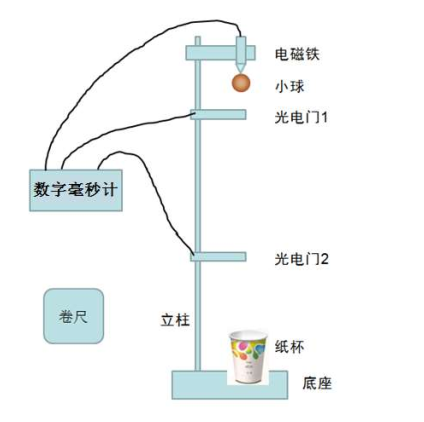
\includegraphics[scale=0.8]{zylt.png}
    \caption{自由落体法实验装置}
\end{figure}
\subsection*{三.实验步骤}\noindent
1.调节底座螺栓,使得立柱竖直,及铅垂线与立柱平行且恰好通过两光电门中心.\\
2.将数字毫秒计与电磁铁,光电门正确连接,按下开始键释放小球,确保小球能通过光电门中心.\\
3.固定光电门1的位置,调节光电门2到适当位置,测量并记录光电门1,2间的距离$h$.\\
4.释放小球使之自由下落,记录小球通过两光电门的时间差$\Delta t$.\\
5.改变光电门2的位置,重复上述步骤,测量6-8组实验.\\
6.实验结束后将实验器材归位,分析实验数据,作图并拟合,求出重力加速度$g$.
\subsection*{四.数据处理与误差分析}
在实验所得数据中,选取部分合理数据如下:
\begin{center}
    \begin{tabular}{|c|c|c|c|c|c|c|c|c|c|c|c|}
        \hline
        $\Delta t$/ms& 95.1 &95.0&131.1&131.2
                &163.7&163.8&163.9&193.3&220.4&246.1&270.2\\
        \hline
        h /cm &20.00&19.85&29.85&29.87&39.86
                &39.91&39.94&49.95&59.85&69.88&79.94\\
        \hline
        $\overline{v}/m\cdot s^{-1}$ &2.10&2.09&2.28&2.28&2.43&2.44&2.44
        &2.58&2.71&2.84&2.96\\
        \hline
    
    \end{tabular} 
\end{center}
作出散点图,并进行线性拟合,结果如下图:
\begin{figure}[H]
    \centering
    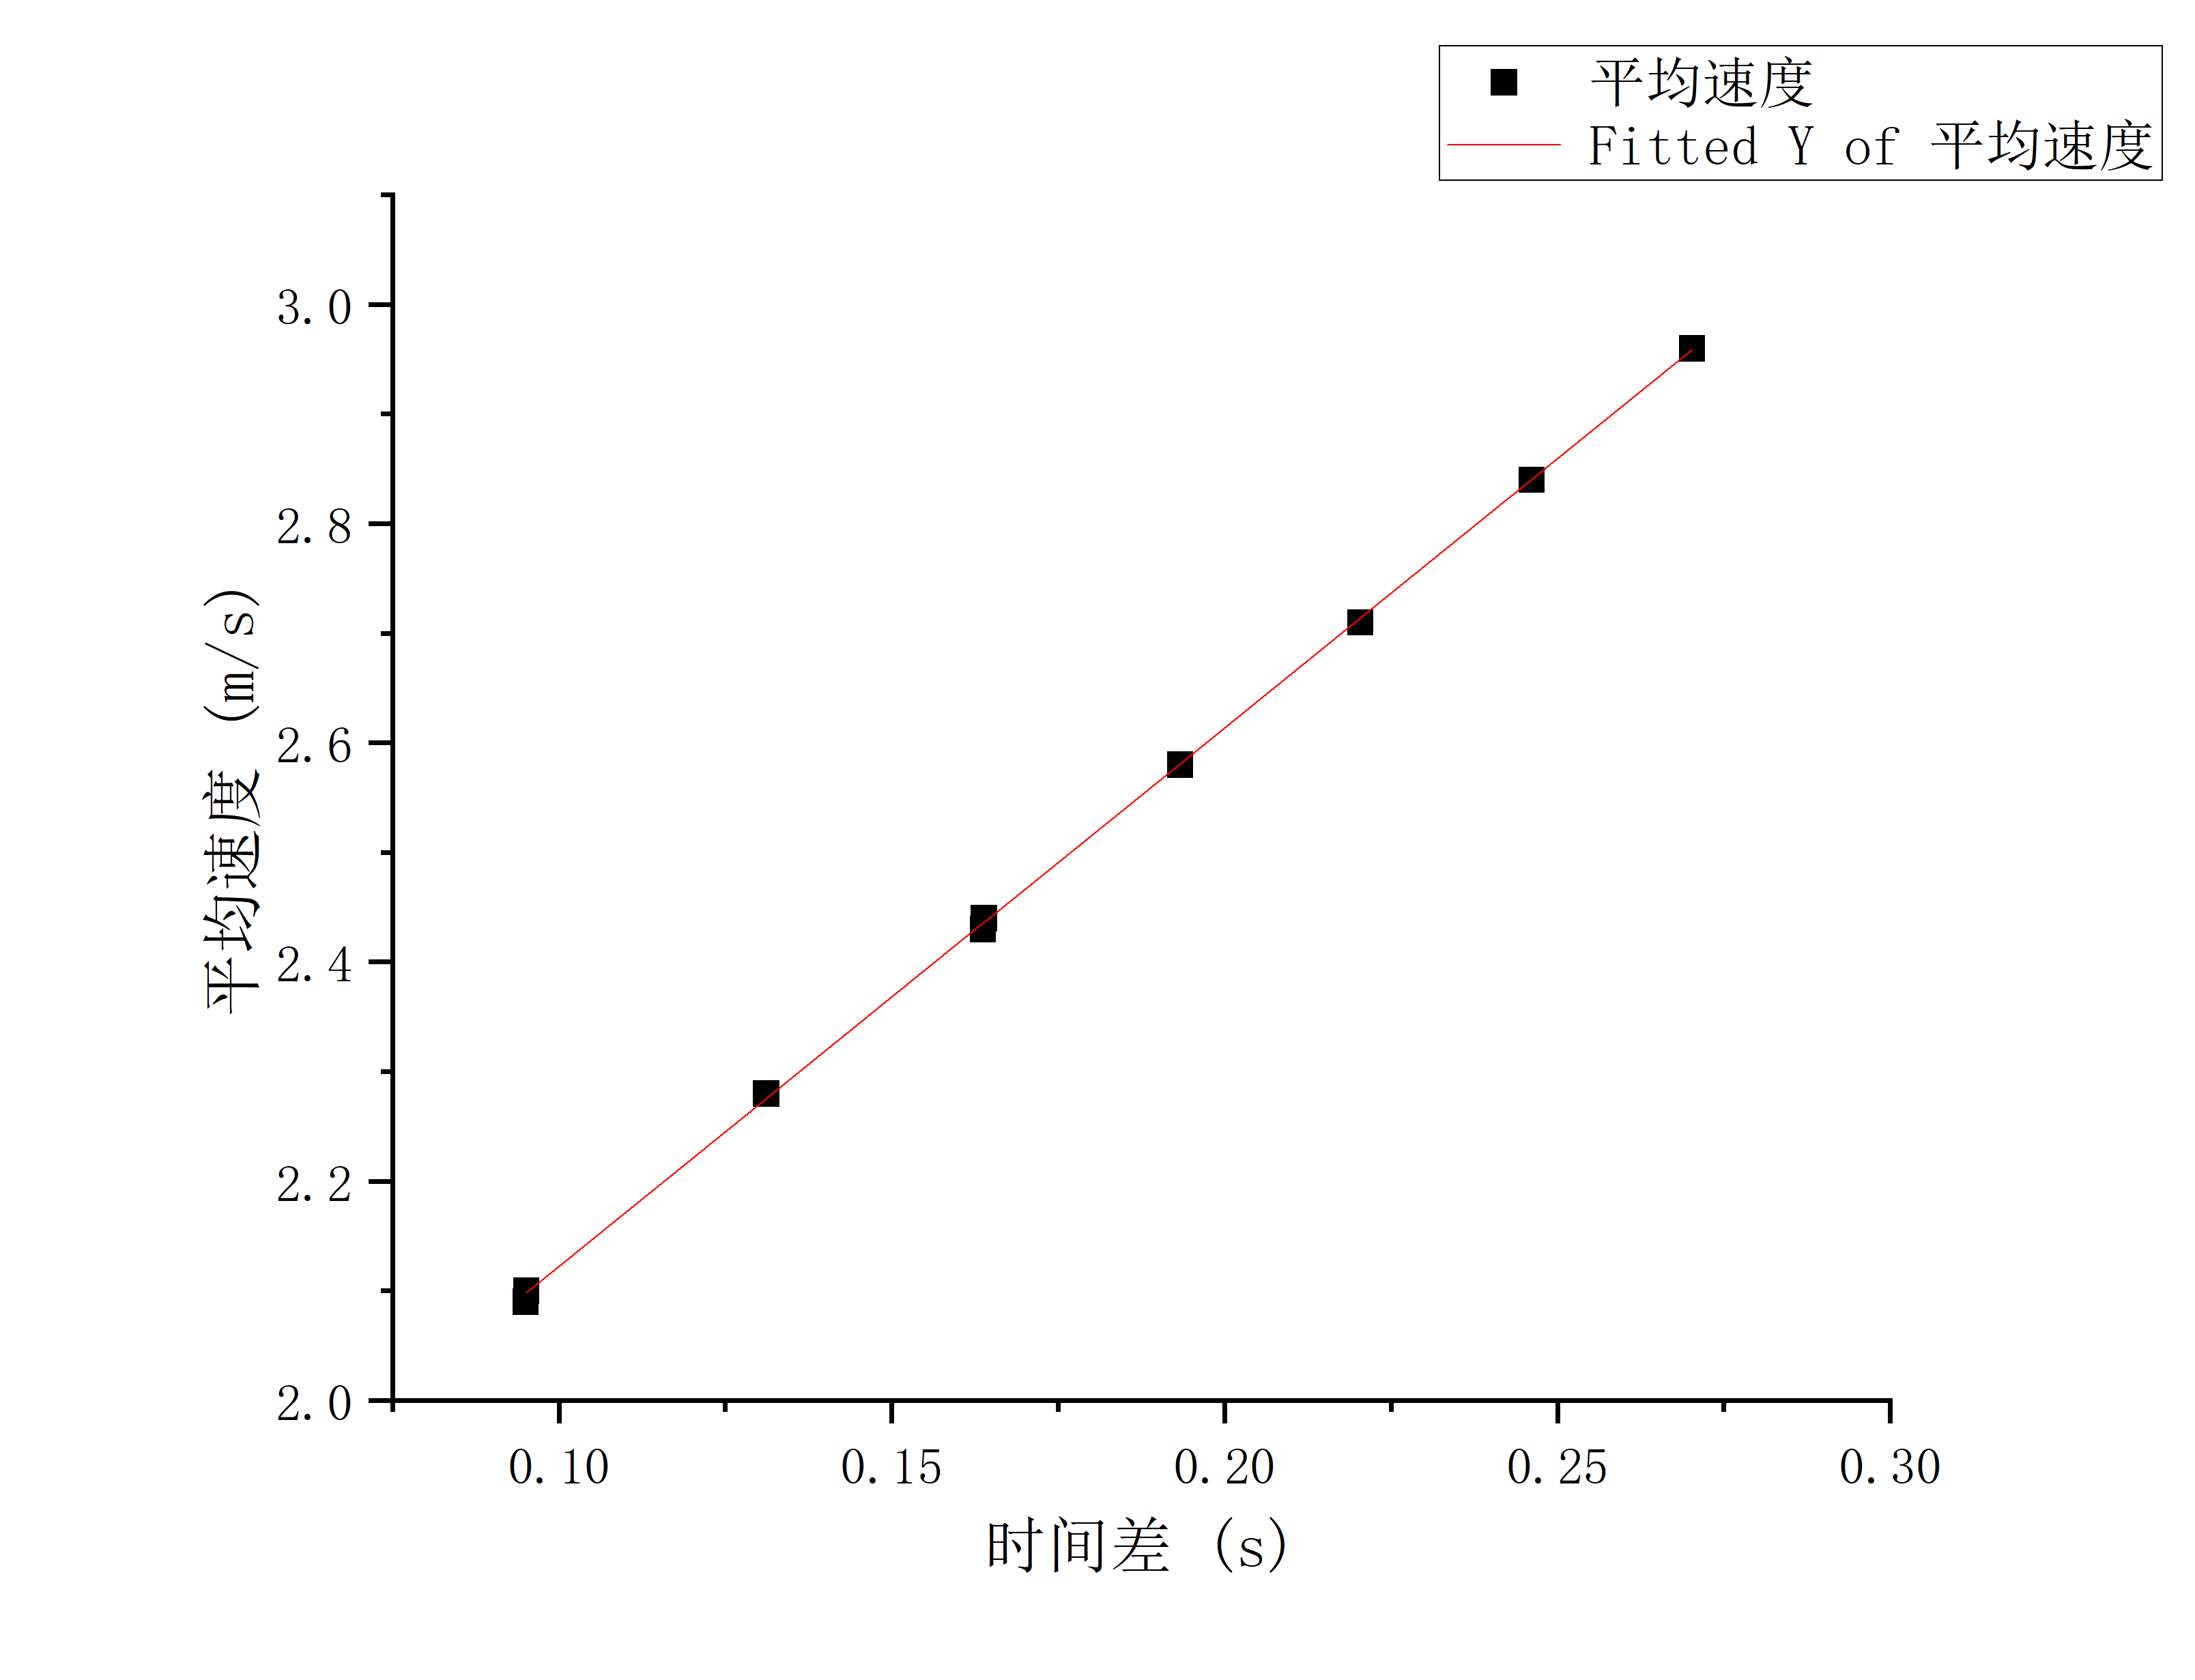
\includegraphics[scale=0.27]{zyltnh.png}
    \caption{自由落体法实验数据拟合}
\end{figure}
实验数据$\overline{v}$与$\Delta t$的皮尔逊相关系数为$r=0.99989$,说明
两者具有良好的线性正相关关系,线性拟合的方程为
$$\overline{v}=1.6313+4.9131\Delta t (m/s)$$
可知重力加速度的值约为$g=9.826m/s^2$\\
误差分析:本实验中的误差有以下几种来源:\\
1.仪器误差:使用卷尺,光电门进行物理量测量时,读数存在一定的误差.\\
2.小球自身的稳定性不同,在下落时可能出现晃动.\\
3.小球下落过程中会受空气阻力作用,对结果产生干扰.\\
4.人为实验操作中存在一定的误差.
\subsection*{五.思考题}\noindent
1.在实际工作中,为什么利用(1)式很难精确测量重力加速度$g$?\\
\indent 公式(1)用于无初速度的下落,且因为计算中需要$t^2$量,对t的测量精度具有较高的
要求,在实际实验中,对t的误差来自两部分:一方面,小球经过光电门的过程中并不能视为质点,其形状
对于t的测量有影响,且这种影响随着$h$的不同即小球的瞬时速度不同而变化;另一方面,电磁铁具有
剩磁,也使得$t$的测量不准确.因此不能用(1)式来测量.\\
\noindent
2.为了提高测量精度,光电门1和2的位置应该如何选取?\\
\indent 对于光电门1,其位置不能离电磁铁即小球的释放位置过近,这是因为
电磁铁的剩磁会影响小球的下落,若距离光电门1过近,则$\Delta t$测量不准;对于光电门2
,其不能距离光电门1过近,因为卷尺测量距离h具有一定的误差,若距离过近,则
误差$\Delta h$会被放大.\\
\noindent
3.利用本实验装置,你还能提出其他测量重力加速度$g$的实验方案吗?
\indent 利用公式$v^2-v_0^2=2gh$,固定光电门1的位置(因而$v_0$保持不变),
改变光电门1,2的间距$h$,测量出小球的半径以及小球每次通过光电门2所用的时间,
并由此计算小球通过光电门2时的瞬时速度$v$,重复多次实验,得到8$\sim$10组数据,做出
$v^2-h$的散点图并进行线性拟合,则拟合图线斜率的一半即为重力加速度$g$.

\section{\Rmnum{4}.单摆法测量重力加速度}
\subsection*{一.实验原理与设计}
理想单摆(没有质量的刚性线,系住一个质点)在真空中由于重力作用而在
与地面垂直的平面内做摆角趋于零的自由振动时,其周期公式为
\begin{equation}
    T=2\pi\sqrt{\dfrac{l}{g}}
\end{equation}
在实际实验中,摆球几何形状,摆线的质量,空气浮力,摆角($\theta<5^{circ}$)
对T的修正小于$10^{-3}$.本实验中,精度要求在$10^{-3}$以内,故上述修正项可以忽略不计,
近似为式(2),并据(2)得
\begin{equation}
    g=\dfrac{4\pi^2l}{T^2}
\end{equation}
利用(3)式,通过测量$l$与$T$,可计算得出重力加速度$g$.
由不确定度均分原理,可得摆长与周期应满足$l>40cm,n>51$,为保证结果精确,实验中取
$l\approx70cm,n=60$(设计过程详见:单摆法测重力加速度实验设计).
\subsection*{二.实验装置}
实验装置如图,所需要的仪器有钢卷尺,电子秒表,单摆(带标尺,平面镜;摆线长度可调)
\begin{figure}[H]
    \centering
    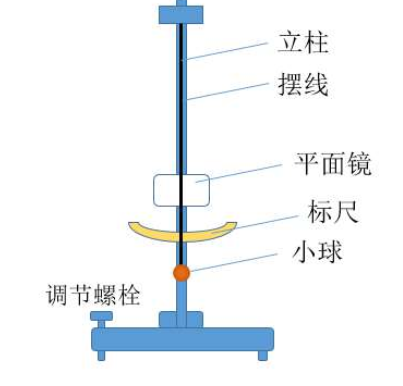
\includegraphics[scale=0.8]{db.png}
    \caption{单摆法测重力加速度实验装置}
\end{figure}
\subsection*{三.实验步骤}\noindent
1.按照实验要求设置好单摆,调节底部螺栓使立柱竖直(三线合一),调整水平,将秒表归零.\\
2.测量摆线长及小球半径,将实际摆长设置为70cm左右.(特别地,在进行实验设计时,我认为应用
游标卡尺测量小球半径,但在实际实验中发现这并不符合最经济原则,因此改为使用卷尺分别测量悬挂点
到小球上端,小球下端的距离,并取平均值作为实际摆长)\\
3.把摆线拉起,取偏离角为$3^{\circ}$,释放小球,当小球经过一个周期后,再次回到最高点时开始计时
(第一周期内有人为释放因素影响,应舍去,从第二周期开始计时),共计数60个周期,小球最后一次回到最高点时,停止计时,记录时间.\\
4.再次测量摆长,确保摆长没有变化.\\
5.重复多次实验,分别记录数据并计算重力加速度.\\
6.实验结束后,将实验器材整理归位,打乱支架平衡,标尺及平面镜位置.
\subsection*{四.数据处理与不确定度分析}
实验中获得的数据如下:
\begin{center}
    \begin{tabular}{|c|c|c|c|c|c|c|}
    \hline
    l/cm&71.25&71.36&71.40&71.40&71.38&71.38\\
    \hline
    n&60&60&60&60&60&60\\
    \hline
    t/s&101.90&101.73&101.51&101.69&101.82&101.85\\
    \hline
    $g/m\cdot s^{-2}$& 9.752&9.800&9.848&9.813&9.785&9.780\\
    \hline
    \end{tabular}
\end{center}
可得$$\overline{g}=9.796m/s^2$$
\textbf{不确定度分析:}\\
对于时间t:
$$u_A=\frac{\sigma_t}{\sqrt{n}}
=\sqrt{\frac{\Sigma_{i=1}^6(t_i-\overline{t})^2}{30}}=0.0574s$$
而$\Delta_{\mbox{仪}}=0.01s$,$\Delta_{\mbox{人}}=0.2s$,
$\Delta_{\mbox{人}}$远大于$\Delta_{\mbox{仪}}$,所以有
$$u_B=\Delta_{\mbox{人}}/C=0.0667s$$
则$$U_t=\sqrt{(t_pu_A)^2+(k_pu_B)^2}=0.429s$$
故对于周期而言$$U_T=\frac{1}{n}U_t=0.00716s$$
对于摆长l
$$u_A=\frac{\sigma_l}{\sqrt{n}}
=\sqrt{\frac{\Sigma_{i=1}^6(l_i-\overline{l})^2}{30}}=0.0232cm$$
而$\Delta_{\mbox{仪}}=0.2cm$,
$\Delta_{\mbox{估}}\leqslant 0.05cm<\frac{1}{3}\Delta_{\mbox{仪}}$,故
$$u_B=\dfrac{\Delta_{\mbox{仪}}}{C}=0.0667cm$$
$$U_l=\sqrt{(t_pu_A)^2+(k_pu_B)^2}=0.252cm$$
由不确定度传递公式,有
\begin{equation}
    \frac{U_g}{g}=
    \sqrt{\left(\frac{U_l}{l}\right)^2+4\left(\frac{U_T}{T}\right)^2}
\end{equation}
可得$\frac{U_g}{g}=0.00914$,故$U_g=0.09m/s^2$,即重力加速度为
$$g=(9.796\pm0.09)m/s^2$$
(4)式表明$\frac{U_g}{g}<1\%$,这说明我们的实验结果达到了实验设计的要求.
\subsection*{五.误差分析与思考讨论}\noindent
\textbf{思考题:分析实验误差的主要来源,提出可能的改进方案}\\
\textbf{误差来源:}\\
1.单摆周期公式使用了一级近似,忽略了摆线质量,空气浮力,摆角等因素影响,导致系统误差.\\
2.秒表,卷尺等仪器使用时存在一定的误差,读数时的人为估算也会产生误差.\\
3.释放小球时,由于外界的微扰,小球可能做微小的圆锥摆而非单摆运动,产生误差.\\
4.实验过程中摆长可能发生变化,产生误差.\\
\textbf{改进方案:}\\
1.在实验允许的范围内,合理地延长摆长,增加所数的周期.\\
2.测摆长时要在竖直平面测量,悬挂点应固定,防止摆长变化.\\
2.选用体积更小,质量更大的小球,减小绳子的质量.\\
3.在释放小球时,用一个平板对小球的运动平面进行限制,避免小球做圆锥摆运动.



\end{document}
